\documentclass[final,twoside,article,10pt]{scrartcl}
%
\usepackage{npac}
\usepackage{amsmath}
\usepackage{url}
\usepackage{graphicx}
\usepackage[utf8]{inputenc}
\usepackage[T1]{fontenc} 
\usepackage[french]{babel}
\usepackage[fixlanguage]{babelbib}
\selectbiblanguage{french}

%
\begin{document}
%
\title{Projet de recherche de L3}
\subtitle{Comparaison de fonctions de hachage}
\author{Florian \textsc{Reynier} \& Mathis \textsc{Caristan}}
%
\date{30/01/2016}

\maketitle

\section*{Résumé }
	\label{sec:resume}
	L'objectif du projet est de comparer différentes fonctions de hachage (non-cryptographique) du point de vue de leur complexité algorithmique et de leur uniformité dans la répartition des clés. On étudiera plusieurs fonctions utilisées couramment en informatique, que l'on testera sur différents fichiers source, de taille et de contenus variables.
	
	
\section{Le hachage}
	%Explications comment, pourquoi ...
	Le hachage est une technologie qui est aujourd'hui cruciale dans le monde de l'informatique, en effet elle est utilisée dans de nombreux domaines comme les bases de données, la programmation, les réseaux \ldots\; Répondre à la problématique est donc intéressant dans la mesure où les résultats peuvent être utiles à tout le monde.\\
	\par Le hachage est un procédé qui utilise une fonction de hachage pour associer à une entrée, une empreinte unique (comme illustré fig \ref{fig:1}). Ceci permet plusieurs applications, notamment un accès rapide à des grandes bases de données, ou d'établir certaines relations (en particulier l'égalité ou la non-égalité) entre des données sans accéder directement à celles-ci. Le hachage permet également de ramener un grand espace de données (potentiellement infini), à un espace d'empreintes fini et de taille connue.\\
	\begin{figure}%[h!]
		\begin{center}
			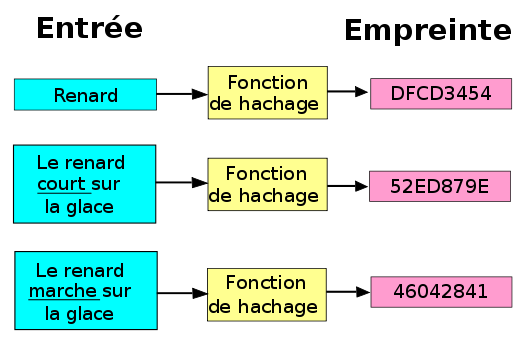
\includegraphics[scale=0.3]{figures/hash}
		\end{center}
		\caption{Illustration d'une fonction de hachage.}
		\label{fig:1}
	\end{figure}\\
	\par Il existe également des fonctions de hachage cryptographique à "sens unique" qui assurent une reconstruction des données impossible par calcul à partir de l'empreinte. Ces fonctions peuvent être utilisées pour vérifier qu'une entrée est associée à une empreinte donnée (dans l'authentification par mot de passe sous UNIX par exemple), mais nous n'étudierons pas ces fonctions dans le cadre de ce projet.
	
	
\section{Méthodologie}
	\subsection{Organisation et outils}
		Pour ce projet, nous allons utiliser OCaml comme langage de programmation. OCaml est un langage performant et 	adapté à ce projet. De plus, c'est un langage que nous ne connaissions pas avant le projet, et sera pour nous l'occasion d'apprendre un nouveau langage. Nous pouvons donc en tirer un double bénéfice.
	Ce projet étant réalisé en binôme, il est nécessaire de pouvoir échanger nos travaux, et gérer les différentes versions le plus simplement possible. Nous allons donc utiliser un système de gestion de version et de code source. Nous avons choisi pour cela Github car c'est une valeur sûre\footnote{https://github.com/Kiskuit/L3Project.git}. Enfin, nous utiliserons \LaTeX pour la production et présentation de fichiers pdf.\\
	\par En ce qui concerne la manière de travailler en groupe, nous prévoyons de nous réunir régulièrement afin d'échanger sur les travaux accomplis depuis la réunion précédente, et de nous répartir les différentes tâches, qui seront ensuite réalisées individuellement.
		
	\subsection{Les fonctions}
		Il nous apparaît évident de premier abord qu'il nous sera impossible de dégager une fonction parmi celles testées comme étant meilleure que les autres à tout point de vue. Il sera donc nécessaire de créer différentes catégories de types de fichiers et de trouver la fonction qui y correspond le mieux, afin de répondre le plus précisément possible au sujet.
		
	\subsection{Les clefs}
		Nous comptons constituer des corpus de différents types de clefs. Les types de clefs que nous envisageons pour le moment sont :
		\begin{itemize}
			\item[$\bullet$]Du texte en français,
			\item[$\bullet$]Du texte en anglais,
			\item[$\bullet$]Du code,
			\item[$\bullet$]Des listes de log,
			\item[$\bullet$]Des clés aléatoires,
			\item[$\bullet$]Des QRcodes,
		\end{itemize}
		Nous constituerons les corpus à partir de sources libres de ces types de données, notamment la base de donnée du projet Gutemberg et de projets sur GitHub. L'enjeu du choix des clé est d'avoir un ensemble le plus hétérogène possible afin que les tests soient les plus complets possible, mais aussi de garder un ensemble de taille raisonnable afin de garder l'exécution des tests simple.
		
	\subsection{Points de comparaison}
		L'uniformité de répartition des clefs (et le nombre de collision créées), ainsi que les vitesses d'exécution des algorithmes basés sur les diverses fonctions seront les points de comparaison principaux sur lesquels nous comptons travailler.

\section{Analyse}
	Pour évaluer la distribution des empreintes sur la taille de l'espace des empreintes, nous allons nous baser sur une analyse statistique des résultats. Dans le cas où une fonction viendrait à s'éloigner d'une distribution uniforme, il sera également possible de réaliser des ajustements de la distribution par différentes fonctions, et de chercher l'origine de cette irrégularité.



\end{document}